\documentclass[12pt]{article}

\usepackage[margin=1in]{geometry}
\usepackage{tikz}
\usetikzlibrary{positioning}

\tikzstyle{replica}=[draw, circle, thick]
\tikzstyle{write}=[-latex, blue, thick]
\tikzstyle{ack}=[-latex, blue, thick, dashed]
\tikzstyle{read}=[-latex, red, thick]
\tikzstyle{version}=[-latex, purple, thick, dashed]

\newcommand{\drawchain}{
  \node[replica] (r0) at (0, 0) {$r_0$};
  \node[replica] (r1) at (1, 0) {$r_1$};
  \node[replica] (r2) at (2, 0) {$r_2$};
}

\newcommand{\oneversion}[3]{
  \begin{tabular}{|l|l|l|}
    \hline
    $#1$ & $#2$ & #3 \\\hline
  \end{tabular}
}

\newcommand{\twoversions}[6]{
  \begin{tabular}{|l|l|l|}
    \hline
    $#1$ & $#2$ & #3 \\\hline
    $#4$ & $#5$ & #6 \\\hline
  \end{tabular}
}

\begin{document}
\begin{center}
  \Large CRAQ Garbage Collection Bug
\end{center}

We describe a very minor bug in CRAQ's garbage collection. Consider the CRAQ
deployment with three replicas shown below, where $r_0$ is the head and $r_2$
is the tail. Initially, all three replicas store a single version (i.e.\
version $0$) of object $x$, which has value a.
\begin{center}
  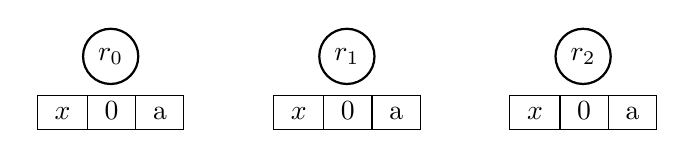
\begin{tikzpicture}[xscale=3]
    \drawchain{}
    \node[below=0 of r0] {\oneversion{x}{0}{a}};
    \node[below=0 of r1] {\oneversion{x}{0}{a}};
    \node[below=0 of r2] {\oneversion{x}{0}{a}};
  \end{tikzpicture}
\end{center}

A client sends a write request with value b to the head, $r_0$. $r_0$ creates a
new version of $x$ and forwards the write request to $r_1$, which also creates
a new version of $x$.
\begin{center}
  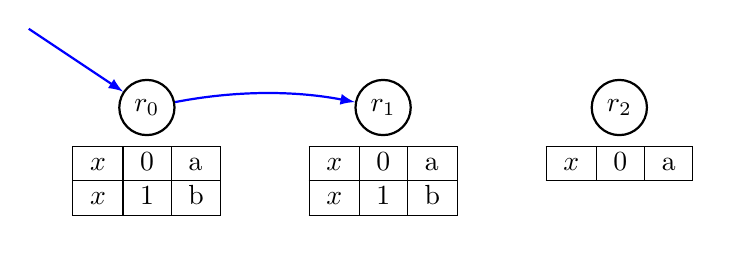
\begin{tikzpicture}[xscale=3]
    \drawchain{}
    \node[below=0 of r0] {\twoversions{x}{0}{a}{x}{1}{b}};
    \node[below=0 of r1] {\twoversions{x}{0}{a}{x}{1}{b}};
    \node[below=0 of r2] {\oneversion{x}{0}{a}};
    \draw[write] (-0.5, 1) to (r0);
    \draw[write, bend left] (r0) to (r1);
  \end{tikzpicture}
\end{center}

Then, a client sends a read request of value $x$ to the head. $r_0$ has more
than one version of $x$, so it cannot perform the read locally. Instead, it
sends a version request to the tail $r_2$. When $r_2$ receives the version
request, it queries to find that its version of $x$ is $0$. It sends $0$ back
to $r_0$, but this message is delayed in network and is not yet received by
$r_0$.
\begin{center}
  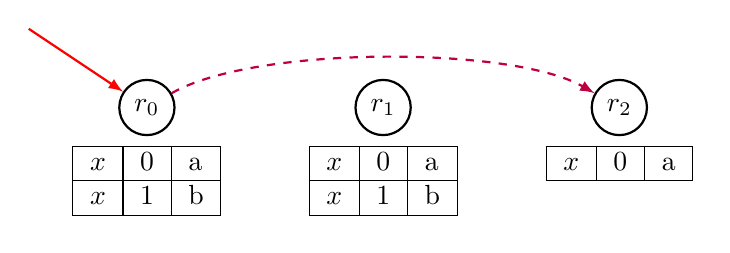
\begin{tikzpicture}[xscale=3]
    \drawchain{}
    \node[below=0 of r0] {\twoversions{x}{0}{a}{x}{1}{b}};
    \node[below=0 of r1] {\twoversions{x}{0}{a}{x}{1}{b}};
    \node[below=0 of r2] {\oneversion{x}{0}{a}};
    \draw[read] (-0.5, 1) to (r0);
    \draw[version, bend left=60] (r0) to (r2);
  \end{tikzpicture}
\end{center}

Next, $r_1$ forwards the write request to the tail, and the tail successfully
propagates write acknowledgements backwards through the chain. When $r_0$ and
$r_1$ receive the acknowledgement, they garbage collect version $0$ of $x$, as
described in the CRAQ paper:
\textcolor{red}{%
``When an acknowledgment message for an object version arrives at a node, the
  node marks the object version as clean. The node can then delete all prior
  versions of the object.''
}
\begin{center}
  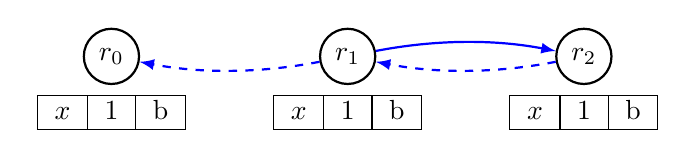
\begin{tikzpicture}[xscale=3]
    \drawchain{}
    \node[below=0 of r0] {\oneversion{x}{1}{b}};
    \node[below=0 of r1] {\oneversion{x}{1}{b}};
    \node[below=0 of r2] {\oneversion{x}{1}{b}};
    \draw[write, bend left] (r1) to (r2);
    \draw[ack, bend left] (r2) to (r1);
    \draw[ack, bend left] (r1) to (r0);
  \end{tikzpicture}
\end{center}

Finally, $r_0$ receives the delayed message, which includes version $0$, from
$r_2$. $r_0$ then attempts to read version $0$ of $x$. The CRAQ paper says
\textcolor{red}{``by construction, the node is guaranteed to be storing this
version of the object''}, but this is not true. $r_0$ does not have this
version (actually, no node has this version), and is stuck.
\begin{center}
  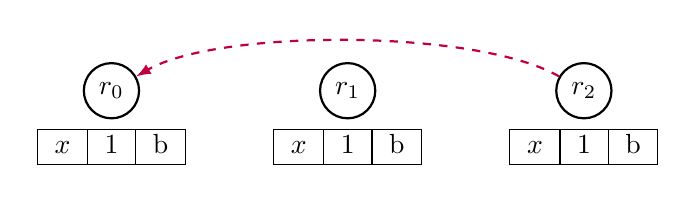
\begin{tikzpicture}[xscale=3]
    \drawchain{}
    \node[below=0 of r0] {\oneversion{x}{1}{b}};
    \node[below=0 of r1] {\oneversion{x}{1}{b}};
    \node[below=0 of r2] {\oneversion{x}{1}{b}};
    \draw[version, bend right=60] (r2) to (r0);
  \end{tikzpicture}
\end{center}
\end{document}
